\documentclass[onecolumn,10pt]{jhwhw}

\usepackage{epsfig} %% for loading postscript figures
\usepackage{amsmath}
\usepackage{graphicx}
\usepackage{grffile}
\usepackage{pdfpages}
\usepackage{algpseudocode}
\usepackage{wrapfig}
\usepackage{pgfplots}
\usepackage{amsfonts}
\usepackage{booktabs}
\usepackage{siunitx}
\usepackage{commath}

% Default fixed font does not support bold face
\DeclareFixedFont{\ttb}{T1}{txtt}{bx}{n}{12} % for bold
\DeclareFixedFont{\ttm}{T1}{txtt}{m}{n}{12}  % for normal

% Custom colors
\usepackage{color}
\usepackage{listings}
\usepackage{framed}
\usepackage{caption}
\usepackage{bm}
\captionsetup[lstlisting]{font={small,tt}}

\definecolor{mygreen}{rgb}{0,0.6,0}
\definecolor{mygray}{rgb}{0.5,0.5,0.5}
\definecolor{mymauve}{rgb}{0.58,0,0.82}

\lstset{ %
  backgroundcolor=\color{white},   % choose the background color; you must add \usepackage{color} or \usepackage{xcolor}
  basicstyle=\ttfamily\footnotesize, % the size of the fonts that are used for the code
  breakatwhitespace=false,         % sets if automatic breaks should only happen at whitespace
  % breaklines=true,                 % sets automatic line breaking
  captionpos=b,                    % sets the caption-position to bottom
  commentstyle=\color{mygreen},    % comment style
  deletekeywords={...},            % if you want to delete keywords from the given language
  escapeinside={\%*}{*)},          % if you want to add LaTeX within your code
  extendedchars=true,              % lets you use non-ASCII characters; for 8-bits encodings only, does not work with UTF-8
  frame=single,                    % adds a frame around the code
  keepspaces=true,                 % keeps spaces in text, useful for keeping indentation of code (possibly needs columns=flexible)
  columns=flexible,
  keywordstyle=\color{blue},       % keyword style
  language=Python,                 % the language of the code
  morekeywords={*,...},            % if you want to add more keywords to the set
  numbers=left,                    % where to put the line-numbers; possible values are (none, left, right)
  numbersep=5pt,                   % how far the line-numbers are from the code
  numberstyle=\tiny\color{mygray}, % the style that is used for the line-numbers
  rulecolor=\color{black},         % if not set, the frame-color may be changed on line-breaks within not-black text (e.g. comments (green here))
  showspaces=false,                % show spaces everywhere adding particular underscores; it overrides 'showstringspaces'
  showstringspaces=false,          % underline spaces within strings only
  showtabs=false,                  % show tabs within strings adding particular underscores
  stepnumber=1,                    % the step between two line-numbers. If it's 1, each line will be numbered
  stringstyle=\color{mymauve},     % string literal style
  tabsize=4,                       % sets default tabsize to 2 spaces
}

\author{John Karasinski}
\title{Homework \# 6}

\begin{document}
%\maketitle

\problem{}
Imagine you had a factorial design in which you were testing if work schedule (none vs. part-time vs. full-time) and course load (part-time vs. full-time) were related to student GPA during an academic quarter. If I told you that this was a balanced design, where each unique combination of conditions (e.g., no work and part-time student status) had 15 participants. What are the df between for each condition, the df for the interaction, the df within (error) and the df total?\\
\\
Taking work schedule as condition A and course load as condition B, we would have:
\begin{align*}
N &= 15 (a \times b) = 15 (3 \times 2) = 90\\
df_A &= (a - 1) = 3 - 1 = 2\\
df_B &= (b - 1) = 2 - 1 = 1\\
df_{AB} &= (a-1)(b-1) = (3-1)(2-1) = (2)(1) = 2\\
df_{error} &= N - (a \times b) = 90 - 6 = 84\\
df_{total} &= (N - 1) = 89
\end{align*}


\problem{}
What are the potential advantages of a factorial ANOVA design? Four are mentioned in your lecture notes. Explain, in your own words, why factorial ANOVA can result in these potential advantages.

\begin{description}
\item[Generalizability] --- In one-way ANOVA, conclusions can be applied only to the groups (levels) of one factor. With factorial ANOVA we can make finer distinctions.
\item[Efficiency] --- We can address several questions with one study.
\item[It is more powerful] --- $MS_W$ is derived from all the cell variances, not just the ones related to only one factor...the error variance is reduced.
\item[Interactions] --- Factorial designs allow examination of interaction effects.
\end{description}

Factorial designs allow us to test multiple factors simultaneously. This is advantageous as it reduces the number of subjects we need to achieve the same power in our tests, as the error variance is reduced. A factorial design approach also reduces the number of experiments we need to run. Instead of conducting a series of independent studies, we are effectively able to combine these studies into one---factorial designs are efficient. The results we find then have a greater generizability, and can give us a broader interpretation of the results. At the same time, factorial designs allow us to look at the interaction of variables. Two variables may interact with each other in ways that were (or were not) anticipated, and factorial ANOVAs give us this information for free.

\problem{}
Give a short example of a hypothetical one-way ANOVA design and demonstrate how a factorial ANOVA design could result in the advantages discussed in question 2.\\

In the lecture notes, we used a one-way ANOVA design around the effectiveness of teaching ANOVA based on the method used to teach. The factor explored was the difference between three example teaching strategies (lecture, discussion, and study). Each subject was rated with a scoring system, and the differences between groups was investigated. To make this a factorial ANOVA design, we could instead investigate both the differences between teaching strategies and the effects of another variable, such as prior experience (yes or no). Using the factorial design, finer distinctions could be made, more questions could be asked with a single study, the error variance would be reduced, and interaction effects could be examined. If, for instance, we had one the one-way ANOVA design described above, the only change in procedure to switch to the factorial design would be asking subjects if they had previous experience. This is a very minor change in experimental procedure (and doesn't really effect the core of the experiment at all). This small change in procedure would lead to us being able to better generalize our results, address multiple questions with a single study, reduce the error variance, and investigate potential interaction effects. Without the factorial design, we would have to run an entire different experiment to investigate the effects of prior experience.

\problem{}
In your own words, describe what simple-effects analyses do and when you would use them?

A simple-effects analysis investigates the existence of an effect for all levels of a factor (e.g., `row effects' or `column effects'). In a two factor ANOVA design based on the previous example, for instance, a simple effect could be the investigation of the best learning strategy for students with or without previous experience. Simple effects use a one-way ANOVA to investigate whether a single factor has an effect when other factors are held constant. Simple effects are often used when an interaction is detected, as blanket statements cannot be made if there is an interaction. In the previous example, suppose that study was very effective for students with previous experience, but not effective for students without previous experience. Using a simple-effects analysis, we could hold the method used to teach factor the same (studying), and investigate whether the difference in effectiveness between students with and without simple effects was statistically significant.

\problem{}
A significant interaction effect suggests that there is a dependency of effect between two conditions. Given this definition, if there is a significant interaction effect does it make sense to interpret main effects of the conditions with the significant interaction? Defend your position (i.e., why or why not).

Main effects should still be (carefully) interpreted despite the presence of a significant interaction. If the main effects are clearly meaningful, then it makes sense to interpret them, whether or not an interaction is present. If, however, the main effect does not really have any meaning, then it should be ignored. Consider Figure 1. Figure 1 represents the result of a factorial ANOVA study testing the main effects of biological sex, lifting condition, and their interaction on percentage of body mass gained. In this analysis, gender, lifting condition, and their interaction were all found to be significant. After a simple-effects follow-up analysis, the workout effect was shown to be significant for males (m), but not for females (f). Despite this, there is a still a main effect of gender. Female's mean percentage of body mass gained is \textit{always} lower than that of males, regardless of workout condition. This is a meaningful effect, and it's important to mention this main effect, regardless of the presence of the significant interaction.

\begin{figure}[h!]
\begin{center}
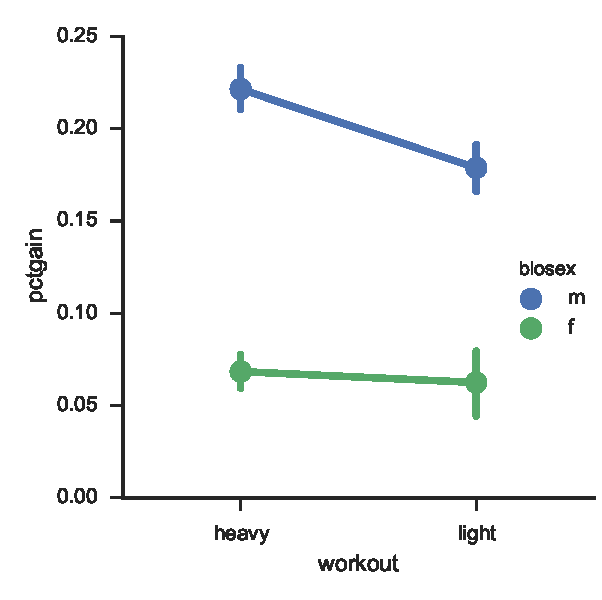
\includegraphics[width=.35\textheight]{p5.pdf}
\label{fig:on}
\end{center}
\caption{Example results with a meaningful main effect and a significant interaction}
\end{figure}

\problem{}
Imagine that you are asked to help analyze some data. A fitness magazine wants to show that women should participate in more intense weight training programs, and that light vs. heavy lifting programs will not cause women to ``bulk up.'' To test this they recruited 60 volunteers to engage in a 60 day transformation program. Half the participants were male, the other half were female. Male and female participants were randomly assigned to participate in either a light or heavy lifting program. The light lifting program focused on endurance---being able to perform more repetitions of the same weight volunteers could lift when they started. The heavy lifting program focused on increasing the maximum amount of weight volunteers could lift---the goal was to increase their starting max by 300\% by the end of the 60 days.
\vspace{1em}\\
1. Descriptive statistics\\
A. Sample Size
\begin{lstlisting}
import pandas as pd
df = pd.read_csv('hw06data.csv')
\end{lstlisting}

\noindent How many volunteers were assigned to each lifting condition overall?
\begin{lstlisting}
res = df.groupby('workout').apply(len)
print("There are {res.heavy} volunteers in the heavy condition and {res.light} volunteers
       in the light condition.".format(res=res))
\end{lstlisting}
\noindent OUTPUT
\begin{lstlisting}[language={}]
There are 31 volunteers in the heavy condition and 29 volunteers in the light condition.
\end{lstlisting}

\noindent How many female volunteers were assigned to each lifting condition?
\begin{lstlisting}
res = df.query('biosex == "f"').groupby('workout').apply(len)
print("There are {res.heavy} female volunteers in the heavy condition and {res.light}
       female volunteers in the light condition.".format(res=res))
\end{lstlisting}
\noindent OUTPUT
\begin{lstlisting}[language={}]
There are 16 female volunteers in the heavy condition and 14 female volunteers in the
light condition.
\end{lstlisting}

\noindent How many male volunteers were assigned to each lifting condition?
\begin{lstlisting}
res = df.query('biosex == "m"').groupby('workout').apply(len)
print("There are {res.heavy} male volunteers in the heavy condition and {res.light} male
       volunteers in the light condition.".format(res=res))
\end{lstlisting}
\noindent OUTPUT
\begin{lstlisting}[language={}]
There are 15 male volunteers in the heavy condition and 15 male volunteers in the light
condition.
\end{lstlisting}
\vspace{1em}
B. Percent Gain Descriptives by Conditions\\
\noindent What are the mean and standard deviation of percent gain overall, for each condition, and for all condition interactions? I recommend making a table of these descriptives.

\begin{lstlisting}
overall = pd.DataFrame({'mean': df.mean(), 'std': df.std()})
overall.index = ['overall']
biosex = df.groupby('biosex').pctgain.agg(['mean', 'std'])
workout = df.groupby('workout').pctgain.agg(['mean', 'std'])
print(pd.concat((overall, biosex, workout)))
print(df.groupby(('biosex', 'workout')).pctgain.agg(['mean', 'std']))
\end{lstlisting}
\noindent OUTPUT
\begin{lstlisting}[language={}]
             mean       std
overall  0.132883  0.073992
f        0.065667  0.026914
m        0.200100  0.032653
heavy    0.142484  0.080641
light    0.122621  0.066012

                    mean       std
biosex workout
f      heavy    0.068438  0.019906
       light    0.062500  0.033741
m      heavy    0.221467  0.023673
       light    0.178733  0.025883
\end{lstlisting}
\vspace{1em}
\noindent 2. State the null and alternative hypothesis for tests of the main effects of biological sex, lifting condition, and their interaction.
\begin{align*}
H_0: \hspace{0.2em} &\alpha_{female} = \alpha_{male} \\
H_1: \hspace{0.2em} &\alpha_{female} \neq \alpha_{male}\\
\hspace{0.2em} &\\
H_0: \hspace{0.2em} &\beta_{heavy} = \beta_{light} \\
H_1: \hspace{0.2em} &\beta_{heavy} \neq \beta_{light}\\
\hspace{0.2em} &\\
H_0: \hspace{0.2em} &\mbox{all } \alpha \beta_{jk} = 0 \left(\alpha \beta_{female/heavy} = \alpha \beta_{female/light} = \alpha \beta_{male/heavy} = \alpha \beta_{male/heavy} =0\right)\\
H_0: \hspace{0.2em} &\mbox{at least one } \alpha \beta_{jk} \neq 0
\end{align*}\\
3.\\
a. Conduct a factorial ANOVA testing the main effect of biological sex, lifting condition, and their interaction.
\begin{lstlisting}
print(anova_lm(ols("pctgain ~ C(biosex)*C(workout)", df).fit(), typ=2))
\end{lstlisting}
\noindent OUTPUT
\begin{lstlisting}[language={}]
                        sum_sq  df           F        PR(>F)
C(biosex)             0.274067   1  404.226801  2.748531e-27
C(workout)            0.008893   1   13.116956  6.310076e-04
C(biosex):C(workout)  0.005066   1    7.471871  8.372369e-03
Residual              0.037968  56         NaN           NaN
\end{lstlisting}

\noindent b. What conclusions do you reach? Explain these in terms of the study. Make sure you incorporate reporting of your statistical analyses into your conclusion.\\

Percentage of body mass gain was subjected to a two-way analysis of variance having two levels of biological sex (female, male) and two levels of workout program (light, heavy). All effects were statistically significant
at the .001 significance level.

The main effect of biological sex yielded an F ratio of $F(1, 56) = 404.2, p < .001,$ indicating that the mean percenteage of body mass gain was significantly greater for males $(M = 0.20, SD = 0.03)$ than for females $(M = 0.07, SD = 0.03)$. The main effect of workout yielded an F ratio of $F(1, 56) = 13.1, p < .001,$ indicating that the mean percenteage of body mass gain was significantly higher for heavy workouts $(M = 0.14, SD = 0.08)$ than for light workouts $(M = 0.12, SD = 0.07)$. However, the interaction effect was also significant, $F(1, 56) = 7.5, p < .001$, indicating that the workout effect was greater in male subjects than in female subjects. The descriptive statistics for these analyses are presented in Table 1. \\

\begin{table}[htdp]
\begin{center}
\begin{tabular}{l r r r r r}
\toprule
Source & SS & df & F & $PR(>F)$ \\
\midrule
Biosex       & 0.27 &  1  & 404.2 & $<.001$ \\
Workout      & 0.01 &  1  & 13.1  & $<.001$\\
Interaction  & 0.01 &  1  & 7.5   & $<.001$\\
Residual     & 0.04 & 56  & & \\
\bottomrule
\end{tabular}
\end{center}
\caption{Factorial ANOVA Results for Fitness Magazine Study}
\end{table}

\noindent 4. Conduct appropriate follow-up analyses. If you had a significant interaction, use simple effects to determine what the effects are of lifting condition based on biological sex. If there was no significant interaction, evaluate any significant main effects of the predictor and IV.
\\
\noindent a. Conduct the appropriate follow-up analyses.
\begin{lstlisting}
print(anova_lm(ols("pctgain ~ C(workout)", df.query('biosex == "f"')).fit(), typ=2))
\end{lstlisting}
\noindent OUTPUT
\begin{lstlisting}[language={}]
              sum_sq  df         F    PR(>F)
C(workout)  0.000263   1  0.355313  0.555909
Residual    0.020743  28       NaN       NaN
\end{lstlisting}

\begin{lstlisting}
print(anova_lm(ols("pctgain ~ C(workout)", df.query('biosex == "m"')).fit(), typ=2))
\end{lstlisting}
\noindent OUTPUT
\begin{lstlisting}[language={}]
              sum_sq  df          F   PR(>F)
C(workout)  0.013696   1  22.263939  0.00006
Residual    0.017225  28        NaN      NaN
\end{lstlisting}

\begin{lstlisting}
print(anova_lm(ols("pctgain ~ C(biosex)", df.query('workout == "light"')).fit(), typ=2))
\end{lstlisting}
\noindent OUTPUT
\begin{lstlisting}[language={}]
             sum_sq  df           F        PR(>F)
C(biosex)  0.097832   1  109.249206  5.450883e-11
Residual   0.024178  27         NaN           NaN
\end{lstlisting}

\begin{lstlisting}
print(anova_lm(ols("pctgain ~ C(biosex)", df.query('workout == "heavy"')).fit(), typ=2))
\end{lstlisting}
\noindent OUTPUT
\begin{lstlisting}[language={}]
            sum_sq  df           F        PR(>F)
C(biosex)  0.18130   1  381.278286  3.140428e-18
Residual   0.01379  29         NaN           NaN
\end{lstlisting}

b. Report your conclusions as you would if you were writing them for a peer reviewed journal. You may use tables to help report your statistical findings if you think it is appropriate. Please make sure your conclusions are in the context of the experimental scenario presented.

An analysis of simple effects showed that workout effect was significant for males, $F(1, 28) = 22.3, p < 0.001$, but not for females, $F(1, 28) = 0.4, p = 0.56$. Therefore, there is no evidence that light workouts differ from heavy workouts for females. An analysis of simple effects showed that the advantage of men over women was significant for both the light workout, $F(1, 27) = 109.2, p < 0.001$, and for the heavy workout, $F(1, 29) = 381.3, p < 0.001$. The descriptive statistics for this analysis are presented in Table 2. From these findings, we can support the fitness magazine's claim that light vs. heavy lifting programs will not cause women to ``bulk up.''

\begin{table}[htdp]
\begin{center}
\begin{tabular}{l r r r r r}
\toprule
Source & SS & df & F & $PR(>F)$ \\
\midrule
\it{Biosex} & & & & \\
\hspace{1em} Female     & 0.00 &  1  & 0.36 & $0.56$ \\
\hspace{1em} Male       & 0.01 &  1  & 22.3 & $<.001$\\
\it{Workout} & & & & \\
\hspace{1em} Light      & 0.10 &  1  & 109.2 & $<.001$\\
\hspace{1em} Heavy      & 0.18 &  1  & 381.3 & $<.001$\\
\bottomrule
\end{tabular}
\end{center}
\caption{Simple Effects Analysis for Fitness Magazine Study}
\end{table}

\end{document}
